\section{Prerequisites}
\label{sec:prerequisites}

  In this section, we will give a brief overview of the terms and definitions
  that we will use throughout this report. These definitions should not be
  considered complete or even absolutely accurate, as they are a personal
  choice of words with the goal of giving the reader an impression of what
  we are talking about.

  \subsection{Neural networks}
  \label{sub:neural_networks}
  
    A \textit{Neuron} is a programmatic structure (or function) that is based
    on neurons inside the brain. In its most basic form, it takes a vector of
    input variables, calculates a weighted sum and applies an activation function
    (typically a sigmoid function like \textit{tanh}).

    A \textit{neural network} is a collection of neurons which are typically
    arranged in layers, where the input of a layer is the output of the
    preceeding one. The output of the last layer is called the output of
    the network.

  \subsection{Recurrent Neural Networks}
  \label{sub:recurrent_neural_networks}
  
    A \textit{recurrent neural network} is a neural network where the
    output of one or more layers is fed back as input to the network
    or a selection of units. This allows the network to make decisions
    based on previous results / events.

  \subsection{LSTM and GRU}
  \label{sub:lstm_and_gru}
  
    The problem with basic RNNs is that they cannot store information for a long time.
    If a recurrent neural network tries to keep a piece of information over a longer
    period of time, it would have to constantly feed it back as input but this would
    suffer from an exponential decay and is therefore not suited for language processing
    where we may need to refer to information that was mentioned a long time ago \cite{hrdipl}, \cite{bengio}.

    Fortunately, Hochreiter and Schmidhuber came up with a solution called
    Long Short-Term Memory \cite{lstm}.  This type of cell possesses an
    extra internal layer that allows it to store information, acting as a
    kind of memory. The output of the cell is then made up of the current
    input and the data that is stored inside. They solve the problem of
    exponential decay by giving a network means to set aside important
    pieces of information and use it later on, without the danger of
    losing it due to decay.  See (\ref{fig:lstm}) for a schematic of the
    internal structure. In short, LSTMs possess so called \textit{gates}
    that determine if and what information is stored. The \textit{forget
    gate} (marked by an '\verb+x+' on the upper line) decides whether or not
    to drop the current memory state and the \textit{input gate} (marked
    by a '\verb|+|') decides which values to add to the current state.

    \begin{figure}
    \begin{center}
        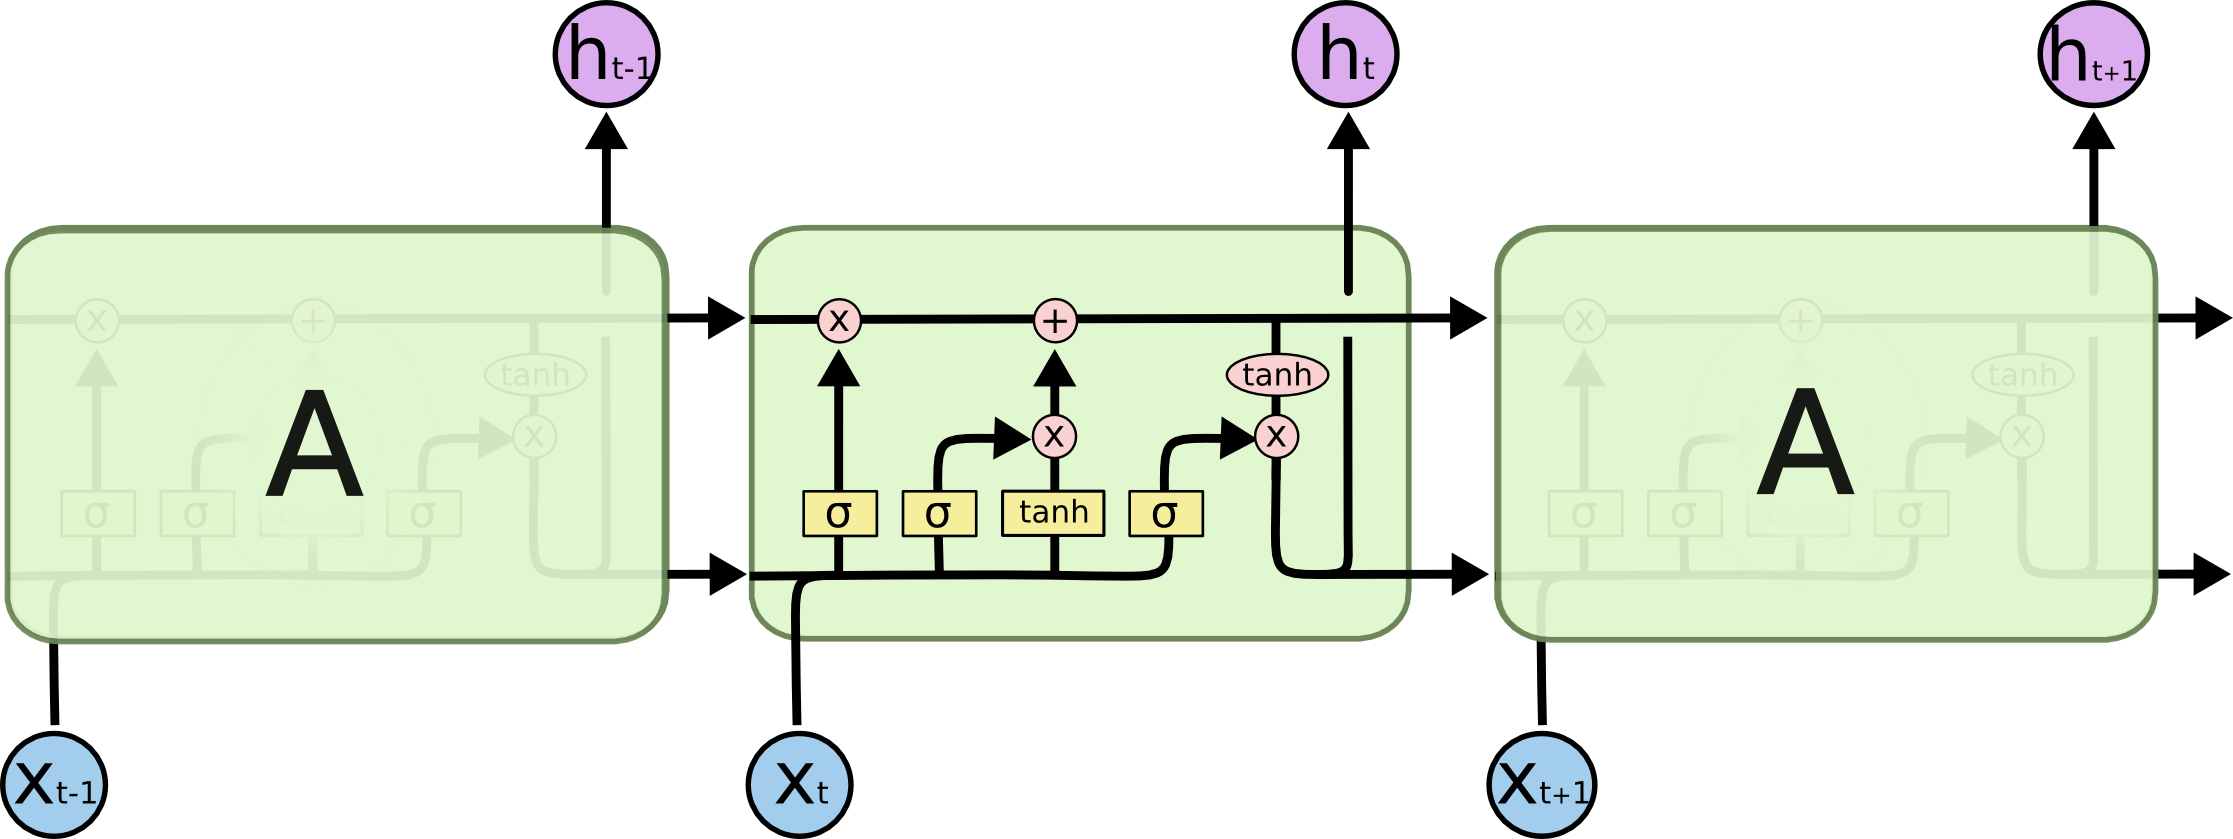
\includegraphics[width=0.9 \linewidth]{lstm.png}
    \end{center}
        \caption{Schematic of an LSTM cell \cite{colah}}
    \label{fig:lstm}
    \end{figure}

	GRUs (Gated Recurrent Units) are a slight simplification of LSTMs \cite{gru}. They
	combine the forget and input gate into a single update gate to reduce the computational workload
	a little bit, but are otherwise essentially the same.
    

  \subsection{Embeddings}
  \label{sub:embeddings}
  
    Usually when solving a multi class classification problem the input and output values are
	represented as one hot encoded vectors. This means that each value $i$ is turned into an
	$n$-dimensional vector where the $i$-th row has a $1$ in it and all other rows are $0$ (where
	$n$ is the number of available classes). When feeding such a possibly huge input vector
	into a layer of a network, that is, multiplying said vector with an $n \times m$-dimensional
	matrix where $m$ is the number of neurons in that layer, one quickly realizes that the result
	of such computation is merely the $i$-th row of that matrix. To reduce the computational
	overhead, it is common to skip the idea of having neurons in such case and simply perform
	a lookup in a huge matrix; the result being an $m$-dimensional vector. This is called an
    \textit{embedding} because the input vector is being embedded in an $m$-dimensional vector space (\ref{fig:embed}).

	If trained correctly, the embedding layer can be used to group words with similar semantics closer
	together while keeping words that have different meaning farther away. The Word2Vec-Model \cite{w2v}
	does this so well that it allows calculations like: \verb|Warsaw - Poland + Germany = Berlin|.

    \begin{figure}
    \begin{center}
        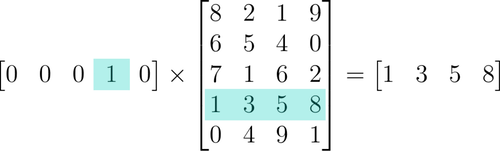
\includegraphics[width=0.8 \linewidth]{lookup_matrix.png}
    \end{center}
    \caption{Example of a lookup in an embedding layer}
    \label{fig:embed}
    \end{figure}
    
	
  \subsection{Keras}
  \label{sub:keras}
  
    Keras is a Python module that contains functions and classes to easily create
    and manipulate neural networks. It contains not only basic neurons, but
    also more involved units like LSTM-Cells or Embedding-Layers (plus
     many more).
